\chapter{Key DESI BAO results}
\label{ch:DESI-key}
\graphicspath{{DESI-key/}}

\section{Introduction}

In this chapter, we provide a summary of major Dark Energy Spectroscopic Instrument results that have relied on the semi-analytical covariance matrices (\cref{ch:RascalC}) and many more supporting studies.
This review will be far from complete and comprehensive, and is influenced by our personal preferences.
E.g., we omitted the neutrino mass problem \citep[see e.g.][]{Y3.cpe-s2.Elbers.2025} because its fair discussion would include much more than BAO.
For the fuller picture, we encourage reading the referenced DESI papers.

Baryon acoustic oscillation (BAO) measurements constrain the expansion of the Universe between now and the emergence of the CMB.
Thus, BAO are very important for understanding the Hubble tension between local measurements and CMB inference.
The expansion history in late times is also the most informative about dark energy evolution because the fraction of dark energy in the total energy budget of the Universe is expected to become low in the far past.

DESI is the most advanced BAO experiment in scientific operation since 2021.
It was designed to measure galaxy redshifts at an unprecedented speed.
During its 5-year program, DESI is scheduled to collect more than 30 million galaxy and quasar spectra, an order of magnitude more than the previous state-of-the-art, SDSS.

\section{Early DESI data (2023)}

The first DESI BAO detection \citep{BAO.EDR.Moon.2023} from the Early DESI data\footnote{The name and some descriptions may suggest that Early DESI data is included in DESI Early Data Release \citep{DESI2023b.KP1.EDR}, but this is not true. The survey validation data comprising the Early Data Release is insufficient for a robust BAO analysis. Instead, the early DESI data represents the first two months of the main survey and is only part of Data Release 1 \citep{DESI2024.I.DR1}.} was a crucial part of the validation of DESI's scientific program \citep{DESI2023a.KP1.SV}.
It confirmed data quality and basic processing choices, abstaining from any cosmological implications.
We found that only the first 2 months of the DESI main survey data already give measurement precision and detection level (shown in \cref{fig:DESI-M2-BAO}) comparable to SDSS-III (DR12) data collected over 6 years \citep{SDSS3-Ross17}.
This confirmed that DESI was on track to reach the planned BAO precision at the end of its full 5-year program.

\begin{figure}[htbp]
    \centering
    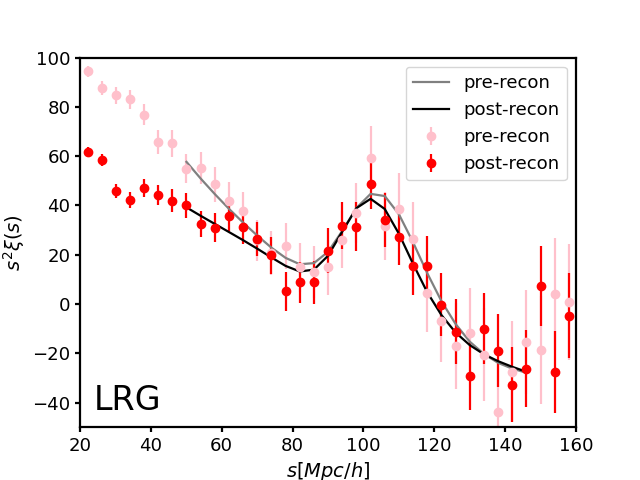
\includegraphics[width=0.495\linewidth]{DESI-M2/plot_BAO_fit_LRG_pre_and_post.png}
    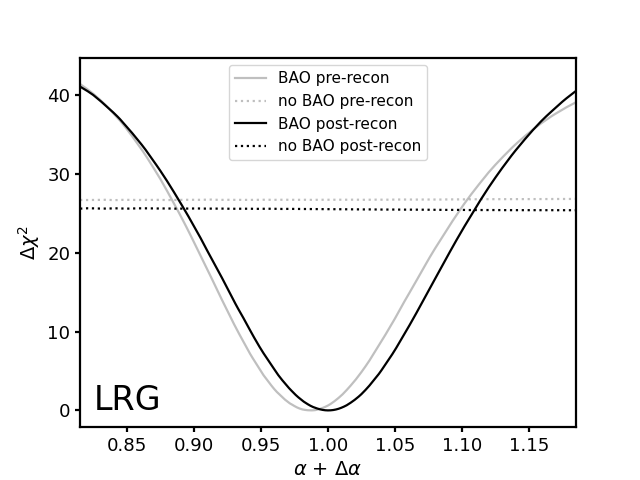
\includegraphics[width=0.495\linewidth]{DESI-M2/plot_significance_alpha_LRG_pre_and_post_rescaled_v2.png} \\
    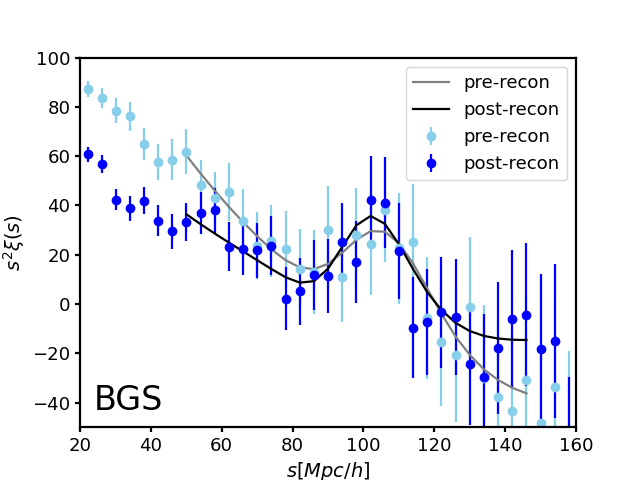
\includegraphics[width=0.495\linewidth]{DESI-M2/plot_BAO_fit_BGS_pre_and_post.png}
    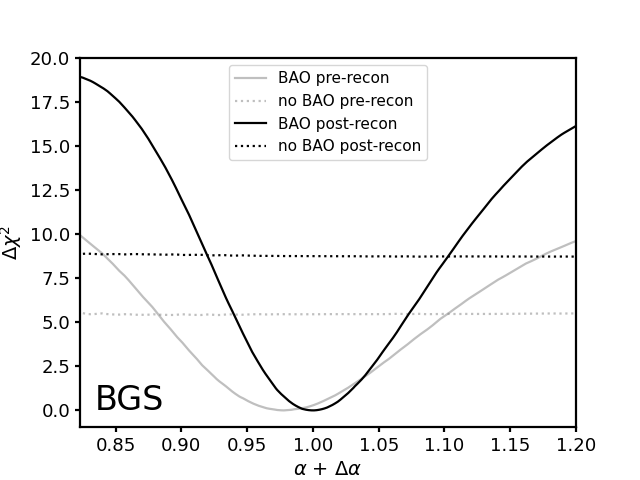
\includegraphics[width=0.495\linewidth]{DESI-M2/plot_significance_alpha_BGS_pre_and_post_rescaled_v2.png}
    \caption[BAO in the Early DESI data]{BAO in the Early DESI data \citep[from the first two months of the main DESI survey, DESI-M2; figure reproduced from][]{BAO.EDR.Moon.2023}.
    Left: measurements and best-fit models before and after standard BAO reconstruction (pre- and post-recon).
    Right: chi-squared differences relative to the best BAO fit in each case.
    In the DESI-M2 LRG sample ($0.4<z<1.1$), the precision of the (isotropic) scale parameter is 1.7\% and the detection is $\approx 5\sigma$; in the BGS sample ($0.1<z<0.5$) --- 2.6\% and $\approx 3\sigma$ respectively.
    Compare LRG to BOSS CMASS ($0.43<z<0.7$) precision of 1.6\% \citep[DR9,][]{BOSS-DR9-clustering}, 1.0\% \citep[DR12,][]{SDSS3-Ross17} and the 0.77\% aggregate precision for LRG from both BOSS and eBOSS \citep{SDSS4-eBOSS-Alam21}; and BGS --- to BOSS LOWZ ($0.15<z<0.43$) precision of 1.7\% \citep[DR12,][]{SDSS3-Ross17}.
    The scale parameter $\alpha$ was shifted by a small value in the spirit of blinding and to discourage premature cosmological inference before the full one-year analysis.}
    \label{fig:DESI-M2-BAO}
\end{figure}

As we mentioned in \cref{ch:RascalC}, our specific contribution has been covariance matrices for the correlation function measurements, crucial for the resulting precision estimates.
For early DESI data, we identified a mismatch in the clustering signal between the simulations and the data, which biased the mock-based covariance.
Using more flexible semi-analytic covariances allowed us to fix this discrepancy at a low cost.

\section{DESI DR1 (2024)}

\subsection{BAO measurements}

To ensure solid cosmological interpretation, the DESI DR1 (2024) galaxy and quasar BAO analysis \citep{DESI2024.III.KP4} involved a thorough re-evaluation of methodology and known systematics.
There largely correspond to a suite of supporting papers on:
theoretical modeling \citep{KP4s2-Chen},
optimal reconstruction \citep{KP4s4-Paillas,KP4s3-Chen},
optimal combination of overlapping tracers \citep{KP4s5-Valcin},
analytical \citep{KP4s8-Alves} and semi-analytical \citep[\cref{ch:RascalC},][]{KP4s7-Rashkovetskyi} covariance matrix validation \citep{KP4s6-Forero-Sanchez},
fiducial cosmology \citep{KP4s9-Perez-Fernandez}
and galaxy-halo connection \citep{KP4s10-Mena-Fernandez,KP4s11-Garcia-Quintero} assumptions.

Many of these supporting studies, as well as the clustering catalog iterations \citep{DESI2024.II.KP3} and the validation of the blinding technique \citep{KP3s9-Andrade} intended to prevent confirmation bias, benefited heavily from our fast, flexible and realistic semi-analytic covariance matrices.
If mock-based covariance matrices were the only option, fully consistent tests of quick corrections, alternative assumptions or differently selected galaxy samples would cost much more time and effort and thus would likely remain unavailable.

\begin{figure}[htbp]
    \centering
    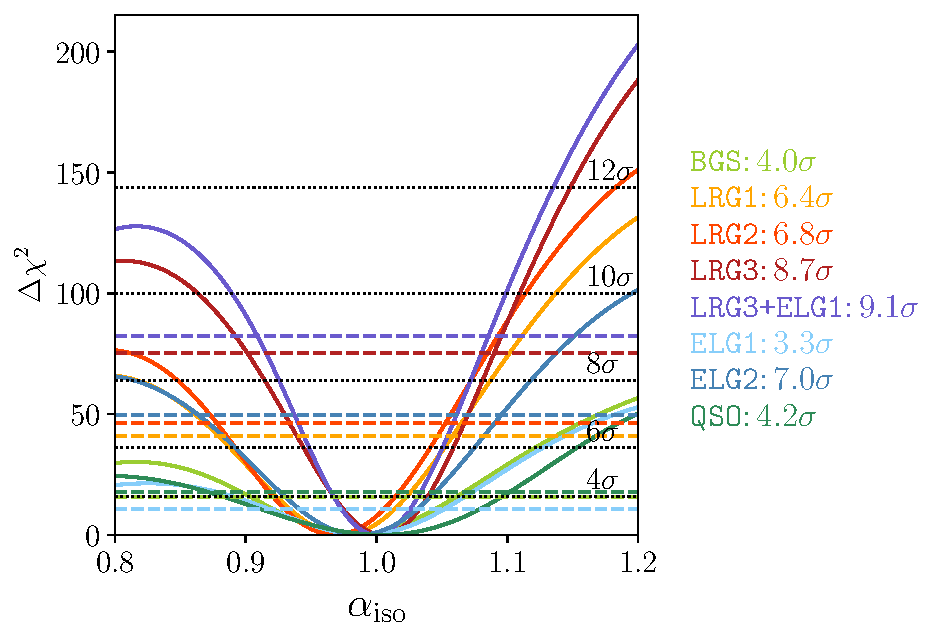
\includegraphics[width=0.6\textwidth]{DR1/bao_detection_level_dr1unblinded.pdf}
    \caption[Detection significance of the BAO features in various DESI DR1 galaxy tracers]{Detection significance of the BAO features in various DESI DR1 galaxy tracers \citep[figure reproduced from][]{DESI2024.III.KP4}.
    Compare with Early DESI Data (\cref{fig:DESI-M2-BAO}).}
    \label{fig:DESI-DR1-BAO-detections}
\end{figure}

We briefly show the impressive detection significances with $\Delta\chi^2$ profiles for DESI DR1 galaxy and quasar BAO in \cref{fig:DESI-DR1-BAO-detections} before shifting attention to the corresponding distance measurements in \cref{fig:DESI-DR1-BAO-diagram}.
The latter also include the Lyman-$\alpha$ forest BAO results from \cite{DESI2024.IV.KP6}.
Their aggregated precision surpassed the previous state-of-the-art by a factor of 1.2\footnote{Although some individual bins (particularly LRG $0.6<z<0.8$, {\tt LRG2}) have a lower precision than optimal BOSS and eBOSS combination \citep{DESI2024.III.KP4,SDSS4-eBOSS-Alam21}.}.
At this accuracy level, hints of deviations from the standard model of cosmology emerged.

\begin{figure}[htbp]
    \centering
    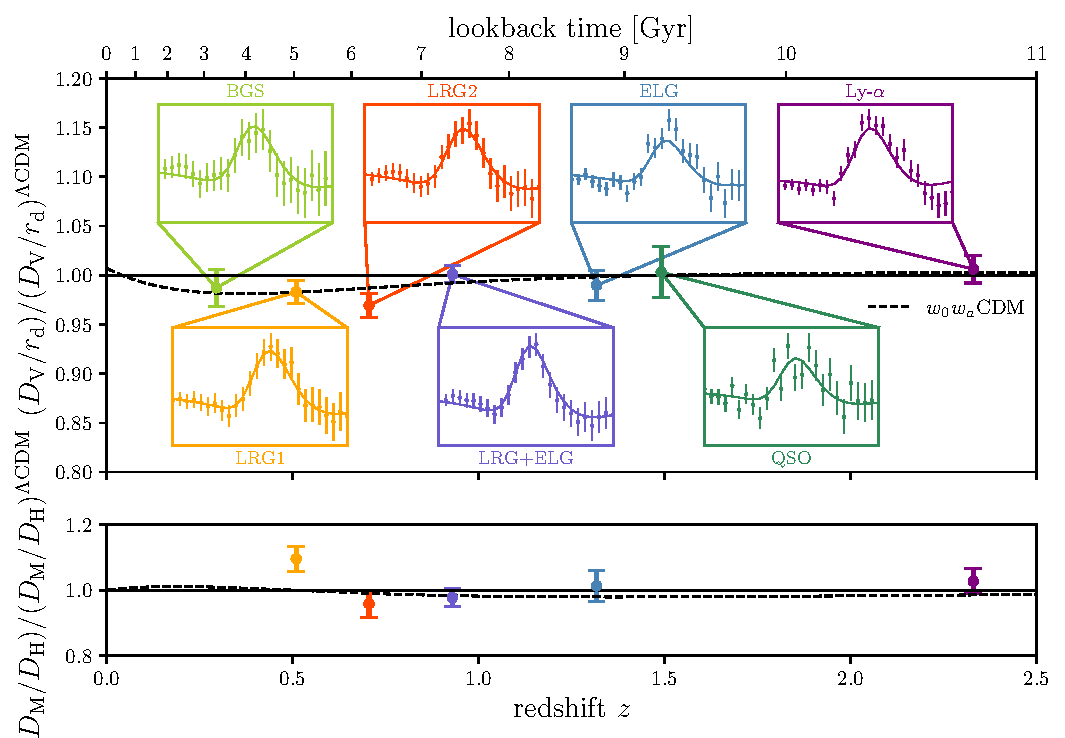
\includegraphics[width=\textwidth]{DR1/bao_isotropic_diagram_z_w0wa.pdf}
    \caption[Summary of DESI DR1 BAO measurements]{Summary of DESI DR1 BAO measurements \citep[figure by Arnaud de Mattia based on][]{DESI2024.III.KP4,DESI2024.IV.KP6,DESI2024.VI.KP7A}.
    All of the errorbars on this plot, except for Ly-$\alpha$, are derived from the \rascalc{} semi-analytic covariance matrices (\cref{ch:RascalC}).
    Improved precision allows us to see deviations from the standard model ($\Lambda$CDM, solid line).
    An alternative dark energy model ($w_0w_a$CDM, dashed line) is preferred.}
    \label{fig:DESI-DR1-BAO-diagram}
\end{figure}

\subsection{Cosmology: dynamic dark energy}

\cite{DESI2024.VI.KP7A} presented implications of DESI DR1 BAO measurements for selected cosmological models.
We choose to highlight the emerging possibility of variable dark energy (\cref{fig:DESI-DR1-w0wa}), in a way similar to recent supernova analyses \citep{PantheonPlus-cosmo,Union3,DES-Y5-SN-cosmo}.
This could become the first confirmed extension to the standard cosmological model, $\Lambda$CDM.

\begin{figure}[htbp]
    \centering
    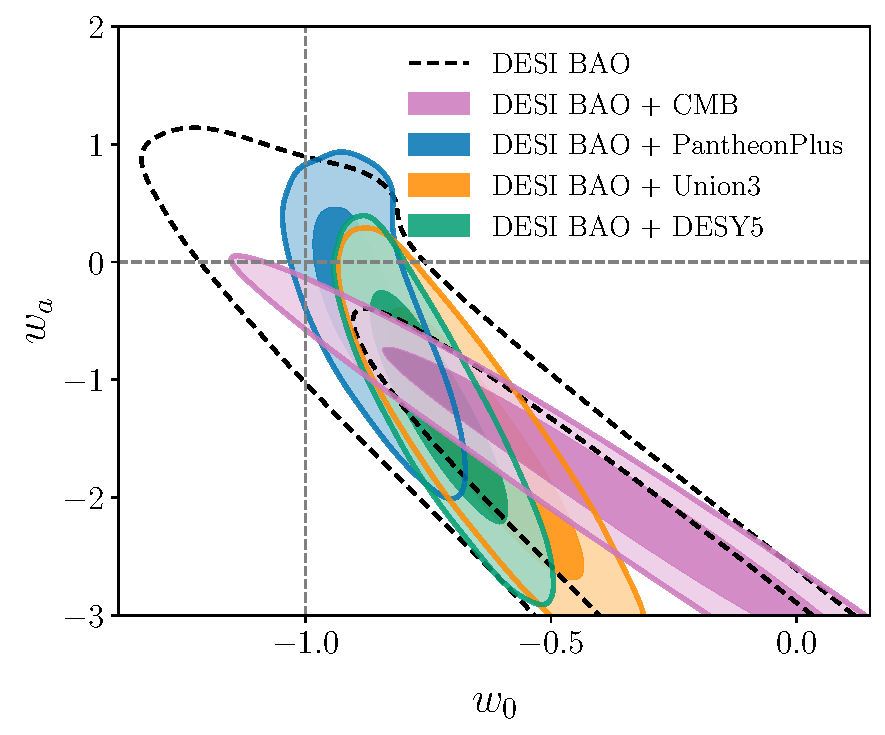
\includegraphics[width = 0.48\columnwidth]{DR1/w0wa_2by2.pdf}
    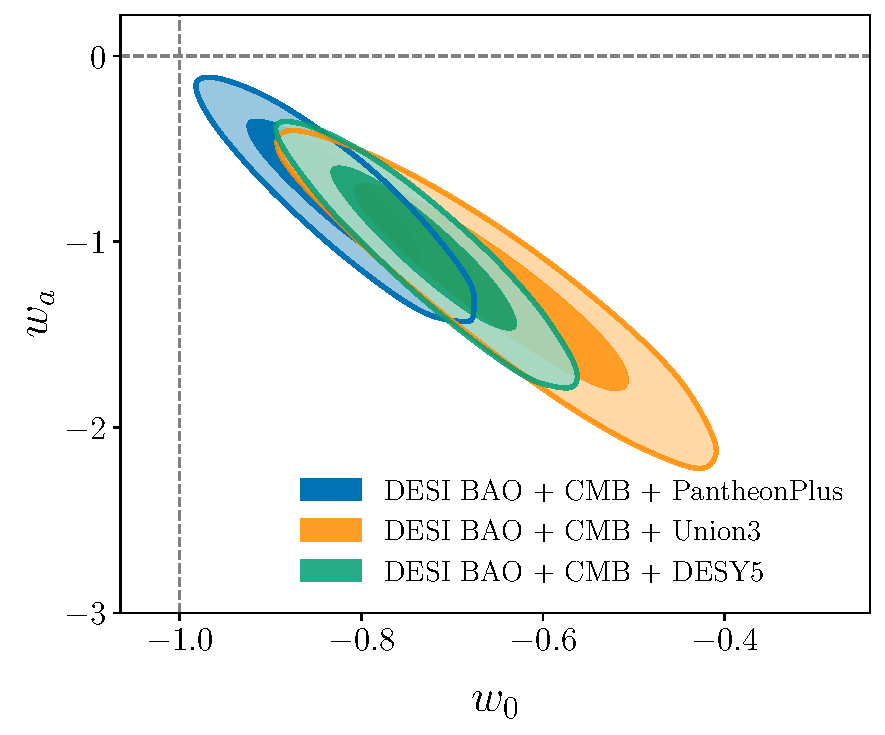
\includegraphics[width = 0.47\columnwidth]{DR1/w0wa_DESI-Planck-SN-95lim.pdf}
    \caption[$w_0w_a$CDM model implications of DESI DR1 data in combination with external datasets]{$w_0w_a$CDM model implications of DESI DR1 data in combination with external datasets \citep[figures reproduced from][]{DESI2024.VI.KP7A}.
    External datasets are CMB (a combination of {\it Planck} PR3 primary temperature and polarization anisotropy power spectra \citep{planck_ttee} and lensing power spectra from {\it Planck} PR4 \citep{Planck-PR4-lensing} and ACT DR6 \citep{ACT-lensing-DR6}) and Type Ia supernovae: PantheonPlus \citep{PantheonPlus-cosmo}, Union3 \citep{Union3} and DES Y5 \citep{DES-Y5-SN-cosmo}.
    DESI DR1 BAO with CMB and different Type Ia supernovae datasets indicate a $2.5\sigma$, $3.5\sigma$ or $3.9\sigma$ deviation from $\Lambda$, the constant dark energy ($w_0=-1, w_a=0$), whereas removing any of them reduces the significance to $\lessapprox 2\sigma$.}
    \label{fig:DESI-DR1-w0wa}
\end{figure}

This analysis assumes the Chevallier-Polarski-Linder (CPL) parameterization of the dark energy equation of state \citep{CPL-Chevalier-Polarski2001,CPL-Linder2003}:
\begin{equation}
    w_{\rm DE} \qty(a) = w_0 + w_a \cdot \qty(1-a).
\end{equation}
The equation of state parameter $w$ drives the density evolution\footnote{Alternatively, $w$ is the ratio of pressure to energy density in a linear equation of state. Assuming no interactions with other components of the Universe, this sets the energy density evolution. But with interactions, the two definitions can differ, then the logarithmic derivative of the density can be called the effective equation of state parameter.} via $\rho \propto a^{-3\qty(1+w)} = \qty(1+z)^{3\qty(1+w)}$, $a$ is the scale factor of the Universe and $z$ is cosmological redshift.
This parametrization is phenomenological, but it can closely reproduce a wide variety of physically motivated models \citep{CPL-Linder2003,CPL-dePutter2008}.
The constant dark energy (or cosmological constant $\Lambda$) have $w_{\rm DE}=-1$ and thus $w_0=-1,w_a=0$.

Interestingly, DESI DR1 BAO alone and with external datasets (\cref{fig:DESI-DR1-w0wa}) align with a line in $w_0,w_a$ space going through zero with a negative inclination.
\cite{DESI2024-physical-DE} found that it does not correspond to well-known models motivated in fundamental physics, but closely aligns with the ``mirage'' dark energy predicted by \cite{mirage-DE} based on cosmological measurements.
Moreover, it implies phantom dark energy ($w_{\rm DE}<-1$) in earlier cosmic times, which is deemed challenging to model \citep[e.g., in][]{interpreting-DESI-DE-Cortes} or even unphysical \citep[e.g., in][]{physical-phantom-DE-after-DESI} due to its violating the null energy condition, $\rho+p\ge 0$.
Notably, interactions of dark energy with other components of the Universe \citep[e.g., dark matter in][]{interacting-DE-after-DESI} may lead to an increase in dark energy density (``effective'' $w_{\rm DE}<-1$) while $\rho+p\ge 0$ holds.
However, the exact description and fundamental motivation of such interactions may be challenging.
Therefore, the nature of dynamic dark energy seems to remain mysterious.

We do not go into much more detail about DESI DR1 results here because the updated DR2 BAO results are now also available.

\section{DESI DR2 (2025)}

\subsection{BAO measurements}

We have been closely involved in the galaxy and quasar BAO analysis of the DESI Data Release 2 \citep[DR2,][]{DESI.DR2.DR2}, comprised of approximately 3 years of the main survey.
This latest BAO analysis \citep{DESI.DR2.BAO.cosmo,Y3.clust-s1.Andrade.2025} has been largely similar to the DR1 analysis \citep{DESI2024.III.KP4}, reusing the results of its many supporting studies.
However, one of the important differences is that the previously performed tests of semi-analytical and analytical covariances (crucially, \rascalc{} in \cref{ch:RascalC}) allowed us to save considerable time and effort by not waiting for the preparation and calibration of approximate mock suites with a large number of realizations.

\begin{figure}[htbp]
    \centering
    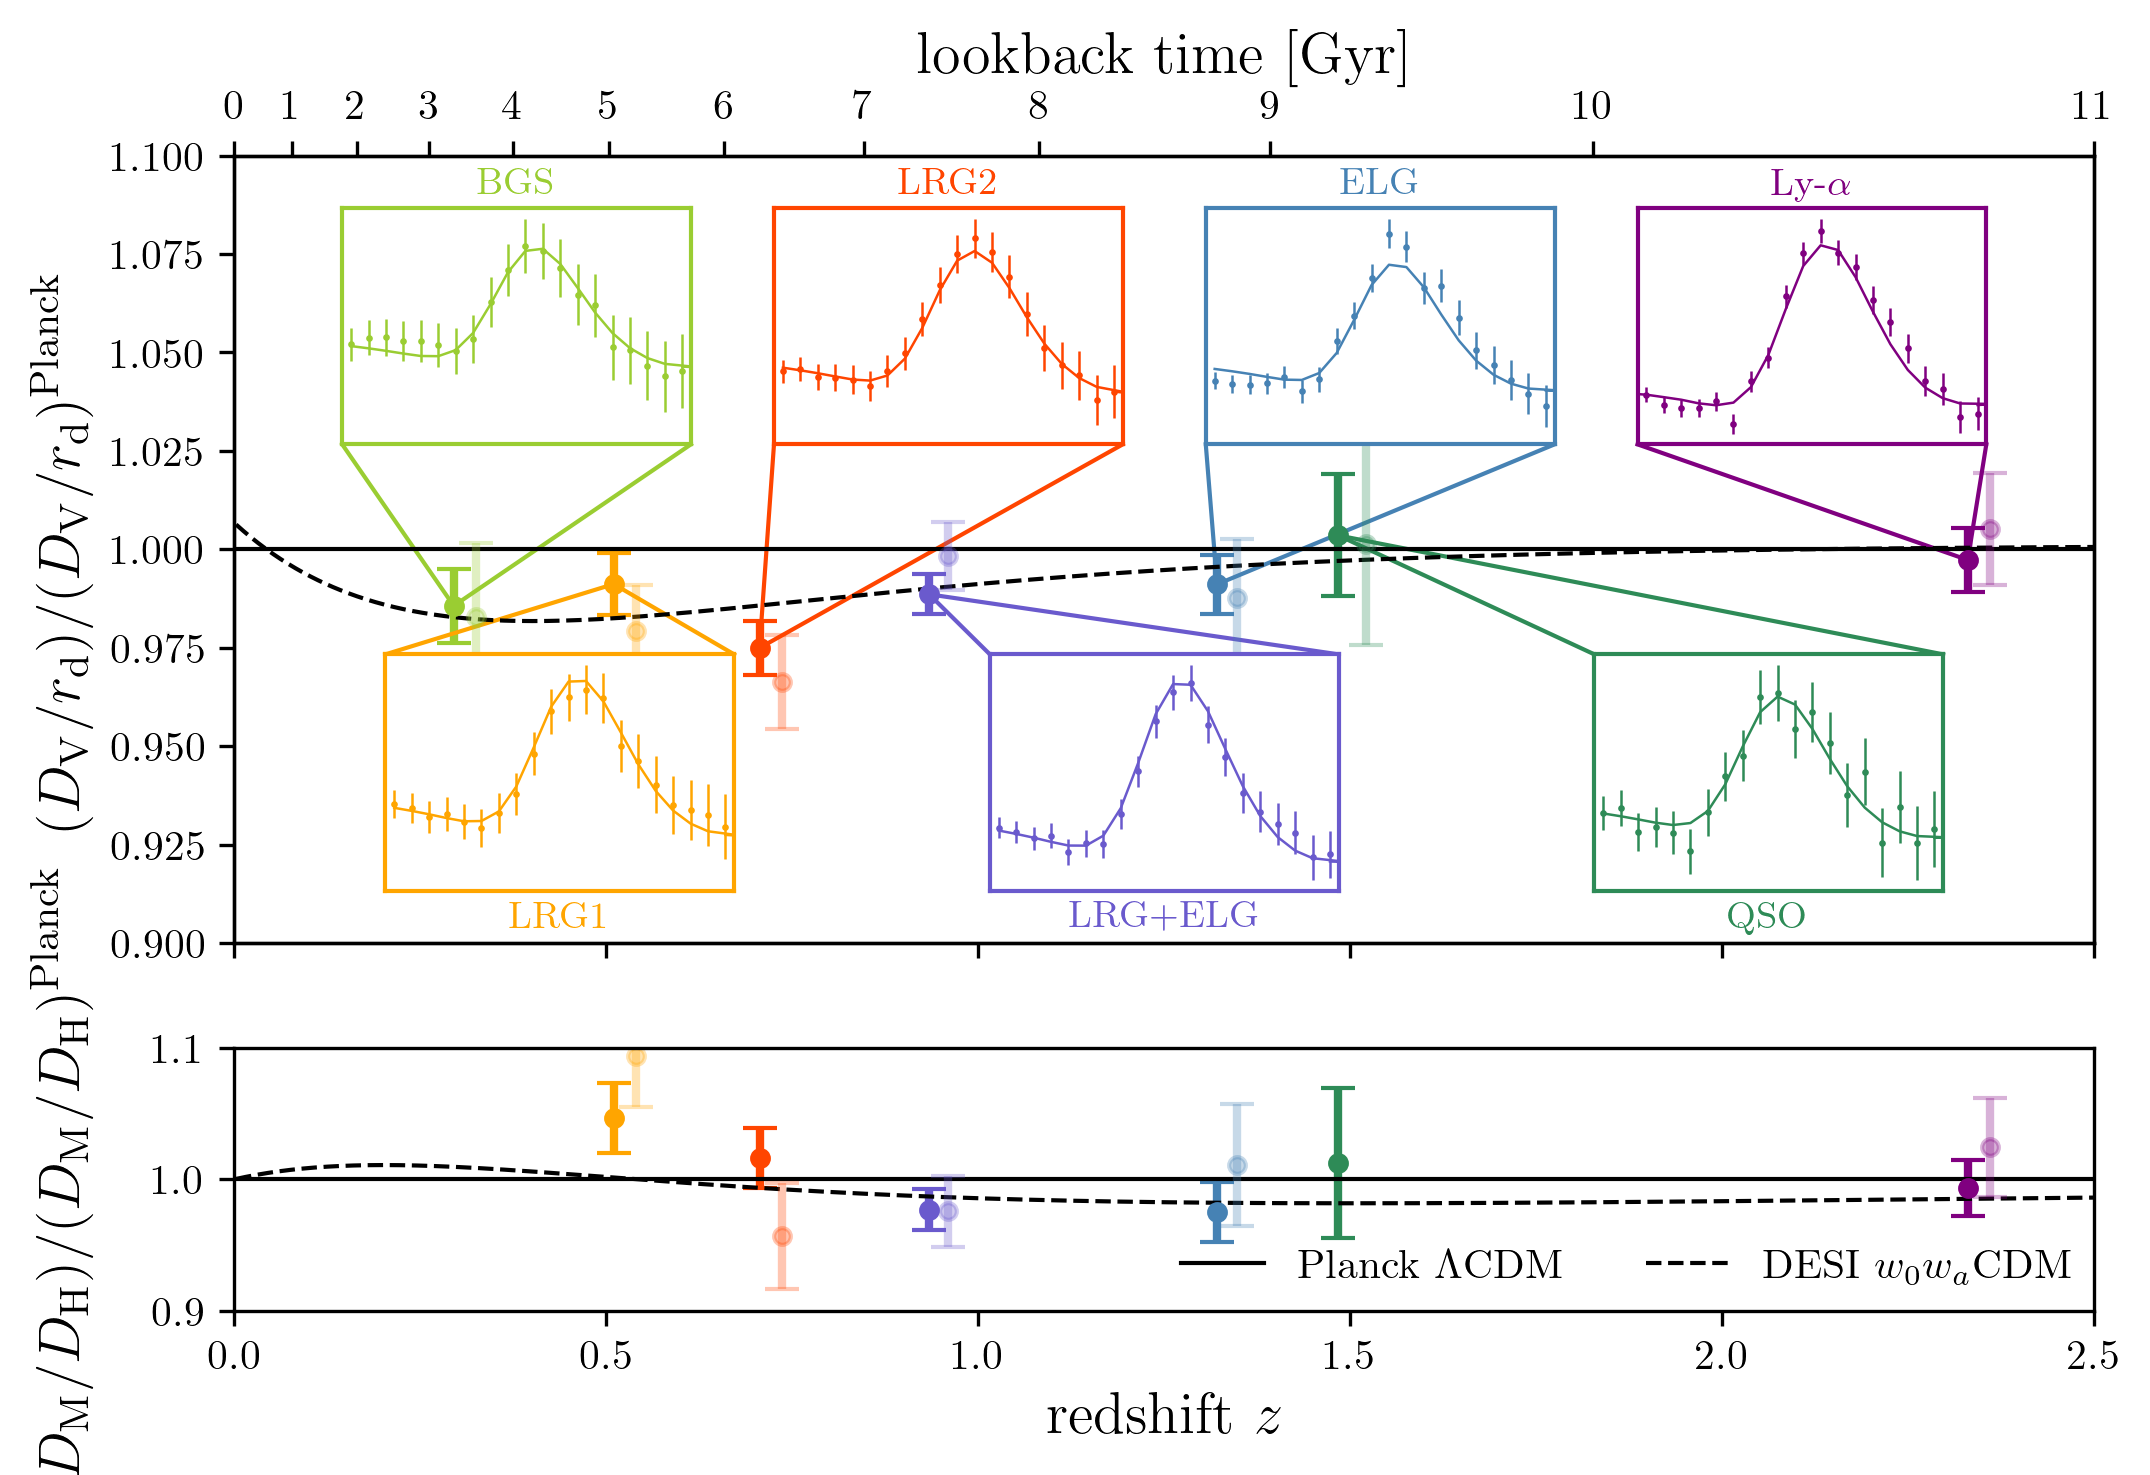
\includegraphics[width=\textwidth]{DESI-key/DR2/bao_measurements_with_y1_diagram_z_fiducial.png}
    \caption[Summary of DESI DR2 BAO measurements]{Summary of DESI DR2 BAO measurements \citep[figure by Arnaud de Mattia based on][]{DESI.DR2.BAO.cosmo,DESI.DR2.BAO.lya,DESI2024.III.KP4,DESI2024.IV.KP6};
    DESI DR1 distance measurements are shown as semi-transparent for comparison.
    All of the errorbars on this plot, except Ly-$\alpha$, are also derived from the \rascalc{} semi-analytic covariance matrices (\cref{ch:RascalC}).
    An alternative dark energy model ($w_0w_a$CDM, dashed line) is still preferred to the standard model ($\Lambda$CDM, solid line) with {\it Planck} parameters \citep{Planck2018-cosmo}.}
    \label{fig:DESI-DR2-BAO-diagram}
\end{figure}

We show a summary of the BAO features and distance measurements in \cref{fig:DESI-DR2-BAO-diagram}.
As before, Lyman-$\alpha$ forest BAO results \cite{DESI.DR2.BAO.lya} are also included.
The precision of all measurements improved, and anisotropic measurement became possible for the second Emission Line Galaxies (ELG) bin\footnote{The first ELG bin is combined with LRG in the main analysis and accordingly this diagram.}.
The precision in all DESI BAO bins now surpasses the BOSS and eBOSS combination \citep{DESI.DR2.BAO.cosmo,SDSS4-eBOSS-Alam21}.
The deviations from the standard model did not disappear in the updated measurements, although several bins shifted closer to it.

\subsection{Cosmological implications}

\begin{figure}[htbp]
    \centering
    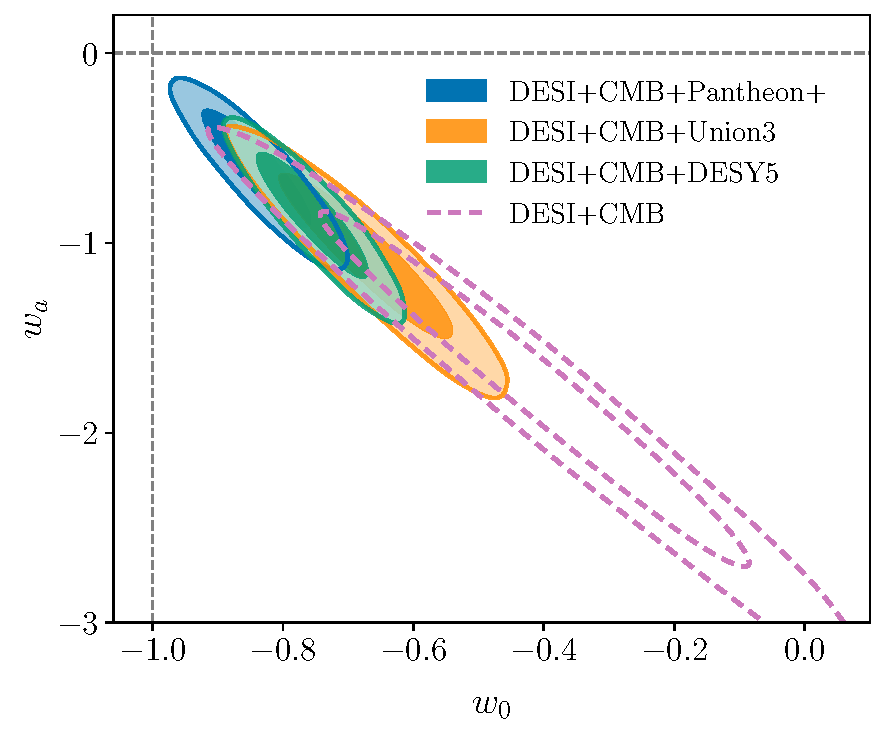
\includegraphics[width=\textwidth]{DR2/w0waCDM_DESI+CMB+SNe_v3.pdf}
    \caption[$w_0w_a$CDM model implications of DESI DR2 data in combination with external datasets]{$w_0w_a$CDM model implications of DESI DR2 data in combination with external datasets \citep[figure reproduced from][]{DESI.DR2.BAO.cosmo}.
    Compared to DR1 in \cref{fig:DESI-DR1-w0wa}, the DESI+CMB+Type Ia SNe contours became tighter but shifted closer to $\Lambda$ ($w_0=-1,w_a=0$), the significance increased slightly to $2.8\sigma$, $3.8\sigma$ and $4.2\sigma$ respectively.
    The DESI+CMB combination is now sufficient to indicate the deviation at $3.1\sigma$.}
    \label{fig:DESI-DR2-w0wa}
\end{figure}

\cref{fig:DESI-DR2-w0wa} presents the DR2 dynamic dark energy ($w_0w_a$CDM) picture.
The constraints based on DESI BAO with both CMB and supernovae improved slightly but shifted closer to the constant dark energy by a similar amount.
The increased precision increased the detection without the Type Ia SNe, with DESI BAO and CMB only, although it is still far from the rigorous threshold of $5\sigma$.
\cite{Y3.cpe-s1.Lodha.2025} conducted an extended analysis of alternative dynamic dark energy parametrizations and non-parametric inference methods, to which we refer an interested reader.

\begin{figure}[htbp]
    \centering
    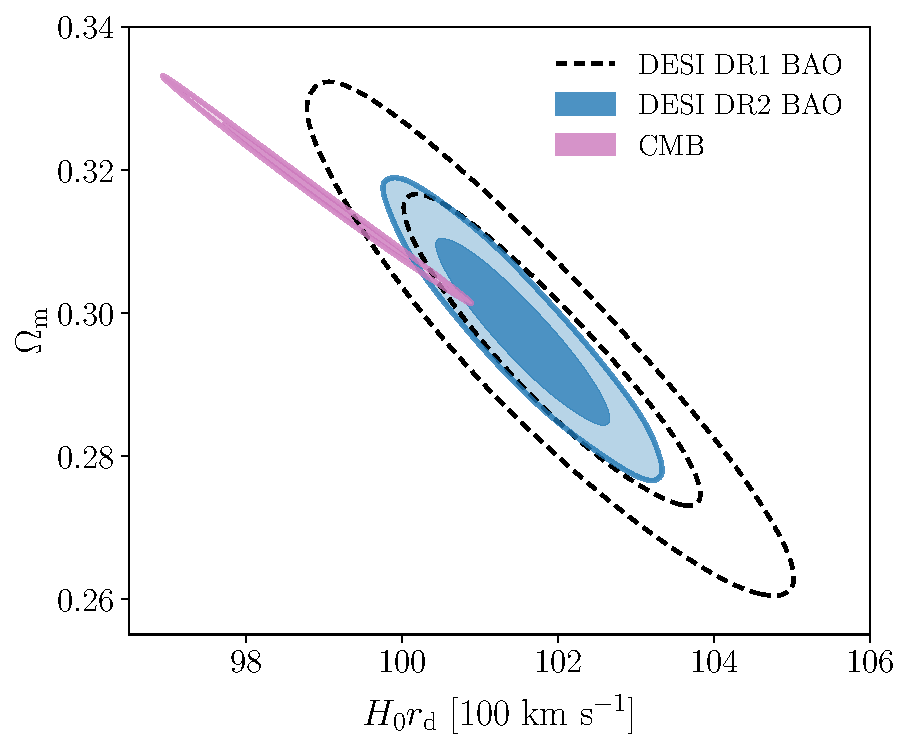
\includegraphics[width=0.495\textwidth]{DR2/LCDM_BAO_v4.pdf}
    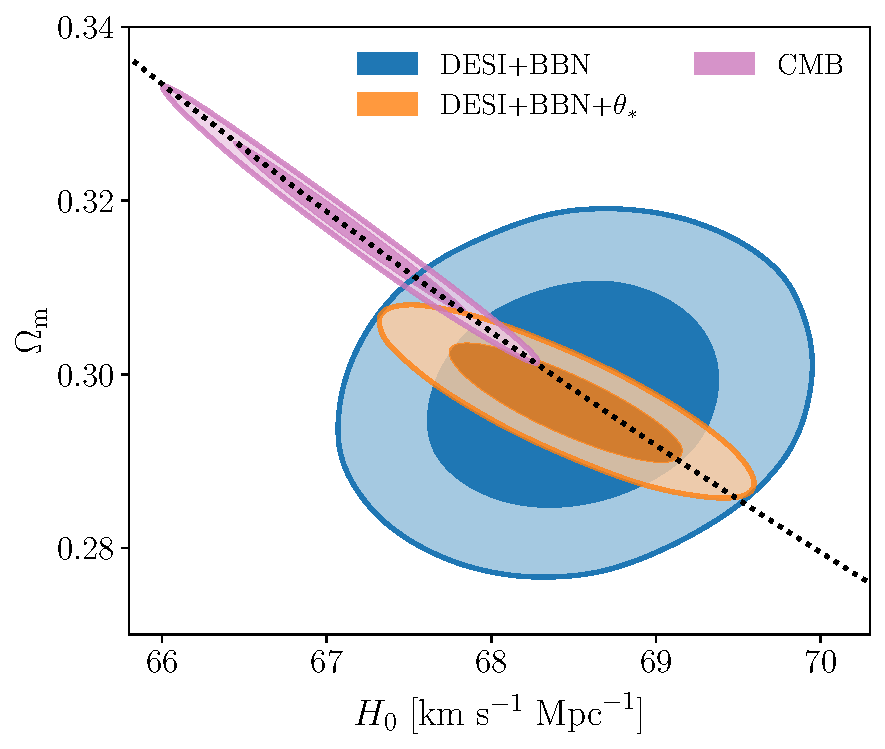
\includegraphics[width=0.495\textwidth]{DR2/LCDM_DESI_calibrated_v4.pdf}
    \caption[Emerging tension identified in $\Lambda$CDM between DESI DR2 BAO and CMB]{Emerging tension identified in $\Lambda$CDM between DESI DR2 BAO and CMB \citep[figures reproduced from][]{DESI.DR2.BAO.cosmo}.
    The left panel shows uncalibrated BAO, from which we can only infer the product of the Hubble constant and the sound horizon $H_0 r_d$.
    The DESI DR2 BAO contour is consistent with DR1, but gives tighter constraints thanks to higher measurement precision, which increases the significance of the discrepancy with CMB from $1.9\sigma$ to $2.3\sigma$.
    The right panel shows the results of sound horizon calibration using the Big Bang Nucleosynthesis \citep[BBN,][]{BBN-2024} alone or together with the angular sound horizon scale $\theta_*$ from the CMB.
    The dotted line shows the degeneracy direction of the CMB.}
    \label{fig:DESI-DR2-LCDM}
\end{figure}

\cref{fig:DESI-DR2-LCDM} shows an emerging tension identified between DESI BAO and CMB in $\Lambda$CDM.
The discrepancy in the matter fraction $\Omega_m$ and the Hubble constant $H_0$ and sound horizon $r_d$ product existed in DR1 at a $1.9\sigma$ level.
In DR2, constraints became tighter and did not shift, increasing the tension to $2.3\sigma$.
After calibrating the sound horizon with the Big Bang Nucleosynthesis \citep[BBN,][]{BBN-2024} alone or together with the angular sound horizon scale $\theta_*$ from the CMB, we infer a higher value of $H_0$ from DESI DR2 than from the CMB.

\begin{figure}[htbp]
    \centering
    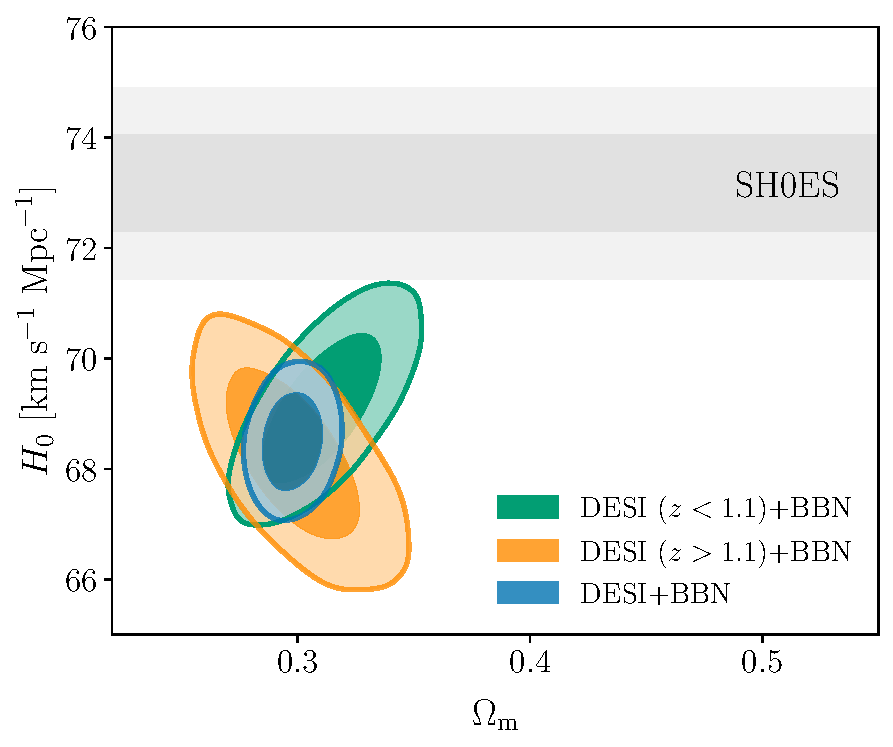
\includegraphics[width=\textwidth]{DR2/DESI_BAO_BBN_tension_SH0ES_v2.pdf}
    \caption[Hubble tension implications of DESI DR2 data]{Hubble tension implications of DESI DR2 data \citep[figures reproduced from][]{DESI.DR2.BAO.cosmo}, using Big Bang Nucleosynthesis \citep[BBN,][]{BBN-2024} for the sound horizon calibration.
    Without CMB, DESI+BBN is now in a $4.5\sigma$ tension with the direct $H_0$ measurement by SH0ES \citep{SH0ES-2022}.
    Even after splitting the DESI BAO measurements roughly in two halves in redshift, each has a $>3\sigma$ discrepancy with SH0ES.
    However, the BBN calibration of the sound horizon assumes standard recombination.}
    \label{fig:DESI-DR2-H0-tension}
\end{figure}

Then it is interesting to compare the Hubble constant inferred from DESI BAO with the direct measurement by SH0ES \citep[which is also famously higher than inferred from the CMB,][]{SH0ES-2022}.
\cref{fig:DESI-DR2-H0-tension} shows that DESI DR2 BAO+BBN $H_0$ is in a $4.5\sigma$ tension with SH0ES.
Unfortunately, dynamic dark energy ($w_0w_a$CDM) does not help to alleviate the Hubble tension, because the inferred Hubble constant value shifts further down \citep{DESI.DR2.BAO.cosmo}.

The inference of the Hubble constant from both BAO and CMB crucially depends on sound horizon calibration, which in turn makes certain assumptions about cosmic recombination.
The physics of recombination has been studied for a long time, and it may be hard to envision a significant deviation from the standard picture.
But \cite{PMF11,PMF13} suggested that primordial magnetic field (motivated in their own right to e.g. seed the galactic magnetic fields) could induce small-scale inhomogeneities in baryons before recombination, which would alter its pace but would not be directly observable in CMB.
This could reduce the sound horizon size and increase the Hubble constant inferred from CMB \citep{JP20} and BAO.
We became interested in this and similar possibilities at an earlier point, which resulted in \cref{ch:H0-clumping} of this thesis \citep[originally published as][]{clumping21}, followed by a summary of more recent developments in \cref{sec:clumping-subsequent}.

\section*{Acknowledgments}

This material is based upon work supported by the U.S. Department of Energy (DOE), Office of Science, Office of High-Energy Physics, under Contract No. DE–AC02–05CH11231, and by the National Energy Research Scientific Computing Center, a DOE Office of Science User Facility under the same contract. Additional support for DESI was provided by the U.S. National Science Foundation (NSF), Division of Astronomical Sciences under Contract No. AST-0950945 to the NSF’s National Optical-Infrared Astronomy Research Laboratory; the Science and Technology Facilities Council of the United Kingdom; the Gordon and Betty Moore Foundation; the Heising-Simons Foundation; the French Alternative Energies and Atomic Energy Commission (CEA); the National Council of Humanities, Science and Technology of Mexico (CONAHCYT); the Ministry of Science, Innovation and Universities of Spain (MICIU/AEI/10.13039/501100011033), and by the DESI Member Institutions: \url{https://www.desi.lbl.gov/collaborating-institutions}. Any opinions, findings, and conclusions or recommendations expressed in this material are those of the author(s) and do not necessarily reflect the views of the U. S. National Science Foundation, the U. S. Department of Energy, or any of the listed funding agencies.

The authors are honored to be permitted to conduct scientific research on I'oligam Du'ag (Kitt Peak), a mountain with particular significance to the Tohono O’odham Nation.